\documentclass{scrartcl}

\usepackage[backend=biber,natbib,style=apa]{biblatex}
\addbibresource{references.bib}

\usepackage[T1]{fontenc}
\usepackage{url}
\usepackage{hyperref}
\usepackage{graphicx}
\usepackage{longtable}
\usepackage{color}
\usepackage{soul}
\usepackage{multicol}

\DeclareRobustCommand{\hlcyan}[1]{\sethlcolor{cyan}\hl{#1}}
\DeclareRobustCommand{\hlcyan}[1]{#1}

\title{lT2216 Assignment 1: Project proposal}
\subtitle{Investigating move reference in the game of go}
\author{Bill Noble}
\date{\today}

\begin{document}

\maketitle

\section{Background: What is go?}\label{background}

Go\footnote{%
In English, go is also known as 
\emph{baduk} (from Korean),
\emph{weiqi} (from Chinese), or
\emph{igo} (from Japanese).
}%
is an ancient abstract strategy board game for two players.
Worldwide, more people play go than any other board game,
though it is most popular in East Asia.

The board consists of grid intersections. 
A \emph{move} consists of placing a stone on one of the available
intersections.
Players alternate turns, placing stones of their color (black or white).
Points are secured by \emph{capturing}
opponent's stones (by completely surrounding an orthogonally connected \emph{group})
and securing \emph{territory} (a region of empty intersections in which
the opponent cannot possibly play without being captured).
When a group is captured,
the stones are removed from the board and play continues.

There are a few more details (the \emph{rule of ko}, for example),
but from this basic rule set, 
enormous strategic complexity emerges.
On the basis of that complexity, 
a distinct culture of go-playing 
has emerged over its more than 2\,500 year history. 

\begin{figure}[h]
  \centering
  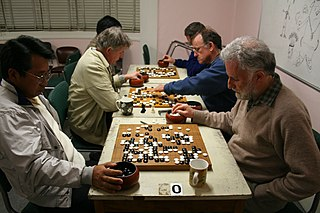
\includegraphics[width=0.6\linewidth]{320px-Go_game_(1907214193).jpg}
  \caption{People playing at a go club in Auckland, New Zealand. Photo: \url{https://commons.wikimedia.org/wiki/File:Go_game_(1907214193).jpg}}
\end{figure}

This project focuses on two aspects of go culture:
\textbf{modes of interaction} 
(ways interacting in the presence of a go board), and
\textbf{move reference}
(ways of talking about different possible next moves).

\section{Modes of interaction}\label{sec:modes}

A \emph{mode of interaction} is related to the idea of a
language game \citep{wittgensteinPhilosophischeUntersuchungenPhilosophical2009}, or
conversational genre \citep{bakhtinSpeechGenresOther1987}.
Although the rules of go specify what game-moves are available to a player
and how to compute the game-effect of a particular game-move
(if the move results in capturing opposing stones, for example),
there are many things about a real-world go-playing interaction that are left
underspecified.
Moreover, there are established ways of interacting
that do not involve playing a game of go \textit{per se},
but that nevertheless 
use knowledge of the rules and shared access to a board
as interactive resources.

\paragraph{competitive play} All of the modes of interaction 
identified here are themselves underspecified in the sense that there 
are additional commonly-understood parameters that affect exactly what kind
of interaction is to take place.
Competitive play is perhaps the most notable example of this.
Competitive games take place on a spectrum from casual to formal.
The most formal competitive games (tournament games, for example),
may explicitly specify additional interaction rules,
such as the use of turn clocks, 
how to take breaks, and
procedures for resolving disputes between players.
In more casual settings (club games, for example),
there are fewer formalized rules around the interaction.
Depending on the conventions of the particular community,
it may be acceptable to have side conversations, 
or even to comment on the game as it is played.

If one of the two players is known to be stronger,
the players may agree to a \textbf{handicap game},
in which some number of the weaker player's stones are placed on the board 
in a particular pattern before play begins.

Other forms of competitive play riff on the two-player paradigm.
In \textbf{simultaneous go}, one (usually stronger) players plays
games against multiple opponents simultaneously.
In \textbf{rengo}, the game is played by two teams of two or more players each.
Players take turns making moves for their team.
In rengo, strategic discussion is typically not allowed within a team, 
but here too different levels of formality may affect what actions are 
considered acceptable.

\paragraph{teaching game} The English-language go wiki 
\textit{Sensei's Library}
describes a teaching game this way:%
\footnote{\url{https://senseis.xmp.net/?TeachingGame}}
\begin{quote}
  A teaching game is a game in which the stronger player teaches the weaker player. Usually their relationship is one of teacher (sensei) and pupil (deshi). The game can be played with full, reduced, or no handicap. The pupil may or may not retake his move. The teacher may or may not give hints as to where to play. The teacher will usually play so as to create instructive situations on the board. The game may or may not be terminated before it is completed. 
\end{quote}

\noindent The article goes on to mention that teaching games may
be provided to a student by a teacher as a paid service.
Here again, the teaching game is a known quantity in the go world,
but the exact parameters of the interaction still 
give room for variation. 

\paragraph{game review} For those who want to improve at go,
game reviews are a way of learning from past games\,---\,%
either one's own or another player's.
A player can review a game solo, 
but game reviews also offer a mode of interaction.
This mode of interaction is different from competitive play and
teaching games because the flow of interaction is not so guided
by the rules of the game itself, though they do 

One typical context for a game review is immediately after 
competitive play. 
One of the players will ask \textit{would you like to review}?
If the other player accepts, 
the two players will typically re-play the game from scratch.
Sometimes one or both of the players will have kept a record,
but often reconstructing the game from memory is part of the 
joint project.
The players will comment on key moves, 
discuss what they were thinking,
and sometimes play out counterfactual variations.
The norms for this mode of interaction are
a subject of discussion in the community.
For example, \textit{Senseis Library}\footnote{\url{https://senseis.xmp.net/?GameReview}}
makes the following recommendation:
\begin{quote}
   Use ``Black'' and ``White'' instead of naming the players or using pronouns. This creates an objective discussion which allows both players to learn without their ego getting in the way. 
\end{quote}

Another type of game review is when a stronger player 
reviews a game with one or both of its players. 
This is common at tournaments and in club play where 
players of various strengths are present.
Like teaching games, game reviews can also be a mode
of interaction in a student-teacher relationship,
and may be provided in exchange for money.

Since the rise of go-playing AI systems, 
it is common to use AI to help review a game,
especially when reviewing solo.
Players can what moves an AI system would have made in a given situation.
However, the raw output can be difficult to interpret.
Why did the system prefer one move over another?
Programs like \textit{KataGo}, \textit{Leela}, and \textit{AI Sensei}
attempt to improve expandability by visualizing different
possible moves and pre-computing the result of short 
follow-up sequences.

Even with these purpose-built programs,
the AI is not engaging in the kind of   
interaction that you would see in a student-teacher
review or in a review between two players who just finished a game.
One eventual goal of this line of work might be to develop
a system that combines a strong go AI with a dialogue system
to interact in that mode.

\paragraph{other modes} There are of course many other
go-based modes of interaction.
If one attends a go tournament or meeting of a go club,
there might be a \textbf{lecture}, 
where a strong player discusses a particular aspect of the game,
sometimes using a large magnetic \emph{teaching board} 
as a communicative resource.
Game \textbf{commentary} takes many forms.
Like with sports, broadcasts of professional sports games
are usually accompanied by expert commentary.
Written go commentaries have been published in newspapers
and magazines for even longer than broadcast media has existed.
The go \textbf{stream} is a new form of interaction,
similar to a video game stream,
in which a player uses a streaming service like Twitch to live-broadcast 
their competitive play against against other people on the internet.
The streamer will usually comment on the game as it is played,
and viewers can interact with the streamer and each other through text chat.

\section{Systems of next-move reference}\label{sec:systems}

As in many \emph{communities of practice} \citep{gumperzSpeechCommunity1972},
go-playing communities have special lexicons of \emph{jargon} 
for referring to game-specific concepts. 
In many western go-playing communities 
(certainly in English and Swedish-speaking communities), 
some of these terms are borrowed from Japanese.

Such jargon appears in many different situations.
A board position might be described as \textit{dangerous for black}.
Taking the other perspective, one might say that 
\textit{whit has good aji} (roughly: potential).
Some players are known to prefer a \textit{fighting game},
while others are more \textit{passive} and prefer to \textit{build}.
In this project, I'm interested in how players refer to 
possible next moves (PNMs).
PNM reference is a communicative affordance used
in several of the modes of interaction discussed in the Section \ref{sec:modes}.
Such references are essential to game review, streaming and commentary,
but can also be found in casual competitive play and in teaching games.
In this excerpt from a go stream, I have highlighted what I think are the
PNM-referring expressions:%
\footnote{%
  Technically this was a pre-recorded video (no interaction with the chat), 
  but the live self-commentary format is one used by many streamers.
  Clip here: \url{https://youtu.be/c2sOdbxVtUA?t=247}}

\begin{longtable}{rl}
 1 & Let’s see what he wants to do.\\
 2 &[Black plays R7]\\
 3 &Ah, he’s playing very \emph{very} close \hlcyan{here}.\\
 4 &That’s a bit too close, so let’s do \hl{\textbf{this attachment}} that I mentioned before \\
     & and see what he wants to do.\\
 5 &[White plays P3]\\
 6 &[Black plays P2]\\
 7 & Ahh I can play \hl{\textbf{this}} [gesture: small circle around Q3] to complete my shape \\
 8 &[White plays Q4]\\
 9 &[Black plays R3]\\
10 & And just \hl{\textbf{extend out}}. \\
11 &[White plays O3]\\
12 &And now I have a (..) [gesture: medium circle around P4] really nice shape \\
     & here as white.\\
12 &[Black plays O2]\\
13 &Hmm (..) I think I’m fine with just \hl{\textbf{extending}} still\\
14 &[White plays N3]\\
15 &[Black plays R10]\\
16 &And there we go, he took his (..) \hlcyan{extension} [getsure: line back and forth R7-R10] \\
   & \hlcyan{a little two-space}.\\
17 & I could probably still leave it if I really wanted to [laughs]\\
     & but this could be a good time to try to make the group strong.\\
18 & You could play \hl{\textbf{R16 here}} to get a base [gesure: medium circle around R14]\\
   & which if you play \hl{\textbf{S16}} you’re basically alive after that. \\
19 & You could \hl{\textbf{attach here}} [gesture: hover R11] to get something.\\
20 & Or you could just \hl{\textbf{jump out}} [gesture: hover O14] (...)\\
     & since it feels like there are so many different options (...)\\
     & you probably still don't really need to do anything here \\
     & [gesture: large circle around Q14]\\
\end{longtable}

\begin{figure}[ht]
  \centering
  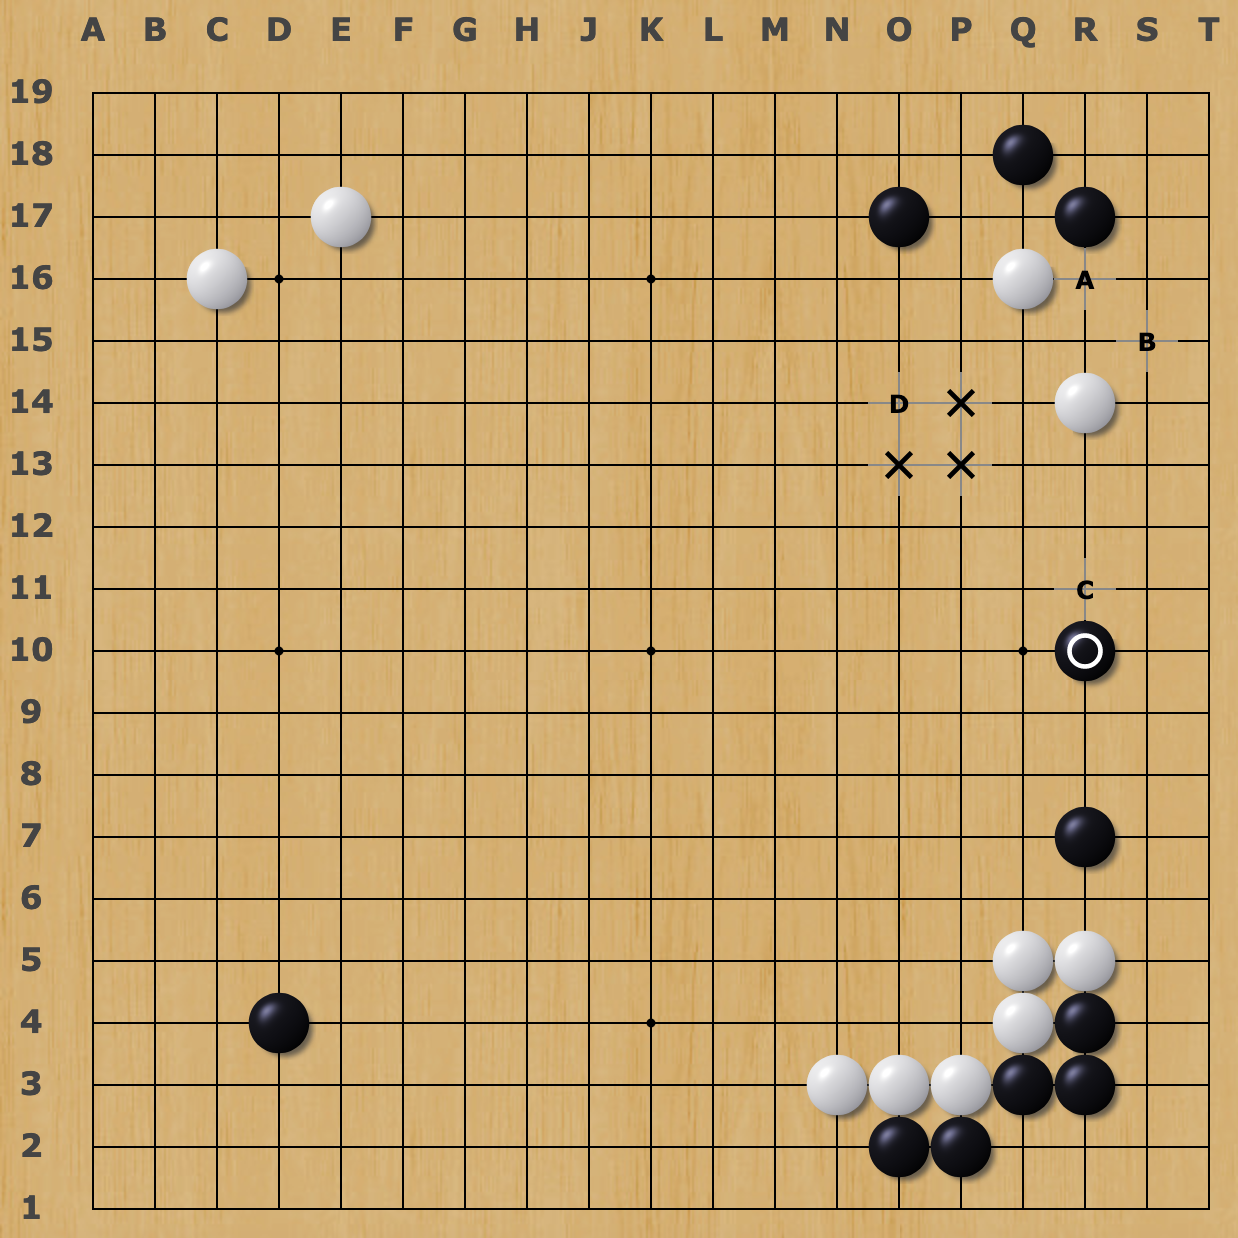
\includegraphics[width=.5\textwidth]{diagram.png}
  \caption{A snapshot of the board state in lines 17--20 of the stream. The (added) marks show the next-move referenants from lines 17--20 as follows: \textbf{A} -- \textit{R16 to get a base}, \textbf{B} -- \textit{S16}, \textbf{C} -- \textit{attach here}, \textbf{D} -- \textit{jump out} (could include moves at any of the \textbf{X}-marked intersections).}
  \label{fig:stream-board}
\end{figure}

\noindent Here are some initial observations:
\begin{itemize}
  \item There are at least three different systems of PNM reference used in this short monologue (those three systems, plus one that isn't used here are detailed below). 
  \item Some referring expressions are ambiguous. 
    In particular, line 20 \textit{jump out} could refer to a few different possible moves in the same small area (see Figure \ref{fig:stream-board}).
  \item Referring expressions are often used in conjunction with gesture (in this case, the gestures are made with a mouse cursor).
  \item Many of the same systems of reference are also used to refer to the opponent's previous move (line 16 \textit{took his extension}, for example). The difference is that previous move reference has the actual move played to draw on as a resource.
  \item Multiple systems of reference can be used at the same time, as in lines 4 and 18.
  %\item It's difficult to cleanly decide what speech refers to a possible move and 
    %what asserts something \emph{about} that which is referred. For example, consider 4 (\textit{this attachment that I mentioned before}) and 18 (\textit{play R16 here to get a base}).
  \item The game state can help to resolve PNM reference, since typically only a small handful of 
    moves are ``viable'', and a good player can quickly narrow down the options.
    This means, however, that the referential potential of an expression can depend on 
    how strong of players the dialogue participants are.
\end{itemize}

\noindent I can identify at least four distinct systems of PNM reference: 

\paragraph{absolute coordinates}

As in line 18, one can use the coordinates labelled along the edge of the board
to name a move by the intersection it would occupy.

Absolute coordinates don't carry meaning like they do in games like chess.
In chess, the E4 square has a particular identity understood in terms of its
strategic value on the board. 
The name \textbf{E4} carries the connotations associated with that identity
and can be used (among experienced chess players) to refer to that square
even if there is no board in the shared context or if the board is not labelled.
In my experience, this is much less the case in go. 
In order for \textbf{R16} to be meaningful, both the speaker and listener
need to have joint attention on a board that is labelled with numbers and letters.
This could be because there are many more intersections in the
standard 19x19 board than there are squares in on a chess board.
Furthermore, the go board has $90^\circ$ rotational symmetry,
meaning that, abstracted away from a particular game state, 
an absolute coordinate referrs to one of (up to) four intersections
with identical strategic value.

\paragraph{corner-relative coordinates}

For this reason, it's also possible to refer to a PNM by its position
relative to the corner.
Conventionally, the corner-most intersection is referred to as \textbf{1-1}.
PNMs at intersections up to \textbf{5-5} are commonly referred to using this system.

Since the corners of the board have special strategic value,
moves near the corners are common in the beginning of the game.
The corner-relative coordinate system is thus associated with
talking about initial corner moves and opening sequences (called \textit{joseki}),
but corner-relative coordinates can also be used to talk about corner play in a particular game.
To use corner-relative coordinates for PNM reference, 
the corner in question needs to be disambiguated by 
context.
This can be communicative context (we were already talking about that corner), 
game state (the corner is \emph{unsettled}, meaning that the active player 
stands to loose out if they don't play there), or both.

\paragraph{demonstratives}

Phrases like \textbf{here}, \textbf{this move}, \textbf{that one}
and so on, are very common for PNM reference. 
These expressions can be anaphoric 
(referring back to a PNM that already been established as a discourse entity),
or by an accompanying gesture. 
Again, the game-state context can also be helpful to disambiguate.

\paragraph{functional descriptors}

I'm calling this category \emph{functional descriptors} because most of 
them refer to PNMs by the move's strategic function or related features.
The following is an exhaustive list of all such expressions I have come
across in the last few weeks (and thought to take note of).
My sense is that all of these terms 
Alternative co-referring forms come after ``;''. 
More specific variants comes after ``--''.

\begin{multicols}{2}
\begin{itemize} 
  \item jump -- one-space jump, two-space jump, ...
  \item extend -- one-space extend, two-space extend, ...
  \item slide -- slide into the corner
  \item cut -- cross-cut
  \item push
  \item peep
  \item crawl
  \item connect
  \item hane -- double hane
  \item attach
  \item capture
  \item atari -- double atari
  \item clamp
  \item pincer
  \item kosumi; diagonal move
  \item block
  \item knight's move; keima
  \item (make a; play the) tiger's mouth
  \item (make an; play the) empty triangle
  \item fix (shape, cutting points)
  \item throw in
  \item defend
  \item approach
  \item escape (to the center)
  \item invade 
  \item enclose (the corner); make an enclosure
  \item threaten to (capture, cut, capture, kill, ladder, ...)
  \item simplify
  \item (make an) exchange
  \item (play the) joseki move
  \item (play the) AI move
\end{itemize}
\end{multicols}

\noindent My sense is that all of these terms get at least some of
their PNM referential potential from community-specific common ground.
That is as opposed to an expression like \emph{the smiley face eye}
which might be used to refer to a PNM that, if played, would be the eye
of a smiley face-like shape on the board.
Such an expression might be understood, but it's not conventional in 
the same way as these are.

What I find interesting about these expressions is that they do more than
just refer\,---\,they say something about the strategic value of the PNM
that is referred to. 
They can carry information about why the speaker might think it is (or isn't)
worth considering the PNM in question, and what the consequences might be for
the continuation of the game.
By using this system of reference, the speaker essentially opens a  
parallel track of communication about PNMs and their strategic value.

Another feature of this system is its ambiguity. 
Because these expressions (with some exceptions) derive their referential
potential from strategic function, they are often ambiguous with respect
to several PNMs.
It's often desirable to refer to any of a collection of PNMs that perform
the same strategic function. Consider line 20, 
which is ambiguous among D or any of the X-marked squares in Figure \ref{fig:stream-board}. 
The speaker uses \textit{jump out}, which is a way of protecting a group of stones from
being captured.
Using this expression is more efficient than saying \textit{O14, O13, P14 or P13},
but it also serves the purpose of communicating the \emph{thought process}
of the speaker.
For that reason, I suspect that functional reference is an important didactic tool,
for teaching and learning the patterns of thought used in to play the game.


\section{Project proposal}\label{sec:proposal}

There basic idea is to implement a system that interacts in one or more 
of the modes of interaction described in Section \ref{sec:modes} 
and that uses one or more of the systems of PNM reference described in Section \ref{sec:systems}.

\begin{itemize}
  \item keep a game state (including aspects that are not visible on the board such as whose turn it is and number of captures)
  \item displayed a shared game board that reflects the game state
  \item ability for both the system and the player to interact with the board
  \item integration with a go engine\footnote{A go engine implements the rules of the game.
      Given a game state, the go engine 
      computes legal next-moves and given a move, it computes the next game state.
      At the end of the game, it may also provide scoring services.
      A go engine is not to be confused with a go AI, which selects among (or provides a ranking of)
      PNMs.}
  \item Integration with a go AI
\end{itemize}

\section{References}
\printbibliography[heading=none]

\end{document}
